\documentclass{article}\usepackage[]{graphicx}\usepackage[]{color}
%% maxwidth is the original width if it is less than linewidth
%% otherwise use linewidth (to make sure the graphics do not exceed the margin)
\makeatletter
\def\maxwidth{ %
  \ifdim\Gin@nat@width>\linewidth
    \linewidth
  \else
    \Gin@nat@width
  \fi
}
\makeatother

\definecolor{fgcolor}{rgb}{0.345, 0.345, 0.345}
\newcommand{\hlnum}[1]{\textcolor[rgb]{0.686,0.059,0.569}{#1}}%
\newcommand{\hlstr}[1]{\textcolor[rgb]{0.192,0.494,0.8}{#1}}%
\newcommand{\hlcom}[1]{\textcolor[rgb]{0.678,0.584,0.686}{\textit{#1}}}%
\newcommand{\hlopt}[1]{\textcolor[rgb]{0,0,0}{#1}}%
\newcommand{\hlstd}[1]{\textcolor[rgb]{0.345,0.345,0.345}{#1}}%
\newcommand{\hlkwa}[1]{\textcolor[rgb]{0.161,0.373,0.58}{\textbf{#1}}}%
\newcommand{\hlkwb}[1]{\textcolor[rgb]{0.69,0.353,0.396}{#1}}%
\newcommand{\hlkwc}[1]{\textcolor[rgb]{0.333,0.667,0.333}{#1}}%
\newcommand{\hlkwd}[1]{\textcolor[rgb]{0.737,0.353,0.396}{\textbf{#1}}}%
\let\hlipl\hlkwb

\usepackage{framed}
\makeatletter
\newenvironment{kframe}{%
 \def\at@end@of@kframe{}%
 \ifinner\ifhmode%
  \def\at@end@of@kframe{\end{minipage}}%
  \begin{minipage}{\columnwidth}%
 \fi\fi%
 \def\FrameCommand##1{\hskip\@totalleftmargin \hskip-\fboxsep
 \colorbox{shadecolor}{##1}\hskip-\fboxsep
     % There is no \\@totalrightmargin, so:
     \hskip-\linewidth \hskip-\@totalleftmargin \hskip\columnwidth}%
 \MakeFramed {\advance\hsize-\width
   \@totalleftmargin\z@ \linewidth\hsize
   \@setminipage}}%
 {\par\unskip\endMakeFramed%
 \at@end@of@kframe}
\makeatother

\definecolor{shadecolor}{rgb}{.97, .97, .97}
\definecolor{messagecolor}{rgb}{0, 0, 0}
\definecolor{warningcolor}{rgb}{1, 0, 1}
\definecolor{errorcolor}{rgb}{1, 0, 0}
\newenvironment{knitrout}{}{} % an empty environment to be redefined in TeX

\usepackage{alltt}
\usepackage[utf8]{inputenc}
\usepackage{hyperref}
\hypersetup{
  linktocpage,
  colorlinks=true, 
  linkcolor=blue,
  citecolor=blue,
  filecolor=blue,
  urlcolor=blue
}
\IfFileExists{upquote.sty}{\usepackage{upquote}}{}
\begin{document}

\begin{knitrout}
\definecolor{shadecolor}{rgb}{0.969, 0.969, 0.969}\color{fgcolor}\begin{kframe}
\begin{alltt}
\hlstd{input_10G} \hlkwb{<-} \hlkwd{read.csv}\hlstd{(}\hlstr{"/home/lucas/ISGlobal/Chip_Seq/DATA/Aligns/q5/10G_in_cov.csv"}\hlstd{,}  \hlkwc{sep} \hlstd{=}\hlstr{"\textbackslash{}t"}\hlstd{,} \hlkwc{quote} \hlstd{=} \hlstr{""}\hlstd{,} \hlkwc{row.names} \hlstd{=} \hlkwa{NULL}\hlstd{,} \hlkwc{stringsAsFactors} \hlstd{=} \hlnum{FALSE}\hlstd{)}
\hlstd{input_1.2B} \hlkwb{<-} \hlkwd{read.csv}\hlstd{(}\hlstr{"/home/lucas/ISGlobal/Chip_Seq/DATA/Aligns/q5/1.2B_in_cov.csv"}\hlstd{,}  \hlkwc{sep} \hlstd{=}\hlstr{"\textbackslash{}t"}\hlstd{,} \hlkwc{quote} \hlstd{=} \hlstr{""}\hlstd{,} \hlkwc{row.names} \hlstd{=} \hlkwa{NULL}\hlstd{,} \hlkwc{stringsAsFactors} \hlstd{=} \hlnum{FALSE}\hlstd{)}

\hlkwd{summary}\hlstd{(input_10G}\hlopt{$}\hlstd{Gene.cov)}
\end{alltt}
\begin{verbatim}
##    Min. 1st Qu.  Median    Mean 3rd Qu.    Max. 
##   0.000   4.868   5.415   5.408   5.725 163.963
\end{verbatim}
\begin{alltt}
\hlkwd{summary}\hlstd{(input_1.2B}\hlopt{$}\hlstd{Gene.cov)}
\end{alltt}
\begin{verbatim}
##    Min. 1st Qu.  Median    Mean 3rd Qu.    Max. 
##   0.000   4.845   5.406   5.370   5.711 136.744
\end{verbatim}
\begin{alltt}
\hlkwd{hist}\hlstd{(input_10G[input_10G}\hlopt{$}\hlstd{Gene.cov} \hlopt{<} \hlnum{10}\hlstd{,]}\hlopt{$}\hlstd{Gene.cov,} \hlkwc{breaks} \hlstd{=} \hlnum{500}\hlstd{)}
\end{alltt}
\end{kframe}
\includegraphics[width=\maxwidth]{figure/unnamed-chunk-1-1} 
\begin{kframe}\begin{alltt}
\hlkwd{hist}\hlstd{(input_1.2B[input_1.2B}\hlopt{$}\hlstd{Gene.cov} \hlopt{<} \hlnum{10}\hlstd{,]}\hlopt{$}\hlstd{Gene.cov,} \hlkwc{breaks} \hlstd{=} \hlnum{500}\hlstd{)}
\end{alltt}
\end{kframe}
\includegraphics[width=\maxwidth]{figure/unnamed-chunk-1-2} 
\begin{kframe}\begin{alltt}
\hlstd{del_10G} \hlkwb{<-} \hlstd{input_10G[input_10G}\hlopt{$}\hlstd{Gene.cov} \hlopt{<} \hlnum{1}\hlstd{,]}\hlopt{$}\hlstd{Gene}
\hlstd{del_1.2B} \hlkwb{<-} \hlstd{input_1.2B[input_1.2B}\hlopt{$}\hlstd{Gene.cov} \hlopt{<} \hlnum{1}\hlstd{,]}\hlopt{$}\hlstd{Gene}

\hlkwd{setdiff}\hlstd{(del_1.2B, del_10G)}
\end{alltt}
\begin{verbatim}
## character(0)
\end{verbatim}
\begin{alltt}
\hlkwd{setdiff}\hlstd{(del_10G, del_1.2B)}
\end{alltt}
\begin{verbatim}
## [1] "PF3D7_0101200" "PF3D7_0300300" "PF3D7_1100100" "PF3D7_1335300"
\end{verbatim}
\begin{alltt}
\hlstd{input_diff} \hlkwb{<-} \hlstd{input_10G[,}\hlnum{2}\hlopt{:}\hlnum{4}\hlstd{]} \hlopt{-} \hlstd{input_1.2B[,}\hlnum{2}\hlopt{:}\hlnum{4}\hlstd{]}
\hlstd{input_diff[}\hlstr{"gene"}\hlstd{]} \hlkwb{<-} \hlstd{input_10G}\hlopt{$}\hlstd{Gene}

\hlkwd{summary}\hlstd{(input_diff}\hlopt{$}\hlstd{Gene.cov)}
\end{alltt}
\begin{verbatim}
##      Min.   1st Qu.    Median      Mean   3rd Qu.      Max. 
## -3.928537 -0.130721  0.009352  0.037974  0.145047 27.356335
\end{verbatim}
\begin{alltt}
\hlkwd{hist}\hlstd{(input_diff[input_diff}\hlopt{$}\hlstd{Gene.cov} \hlopt{<=} \hlnum{5}\hlstd{,]}\hlopt{$}\hlstd{Gene.cov,} \hlkwc{breaks} \hlstd{=} \hlnum{500}\hlstd{)}
\end{alltt}
\end{kframe}
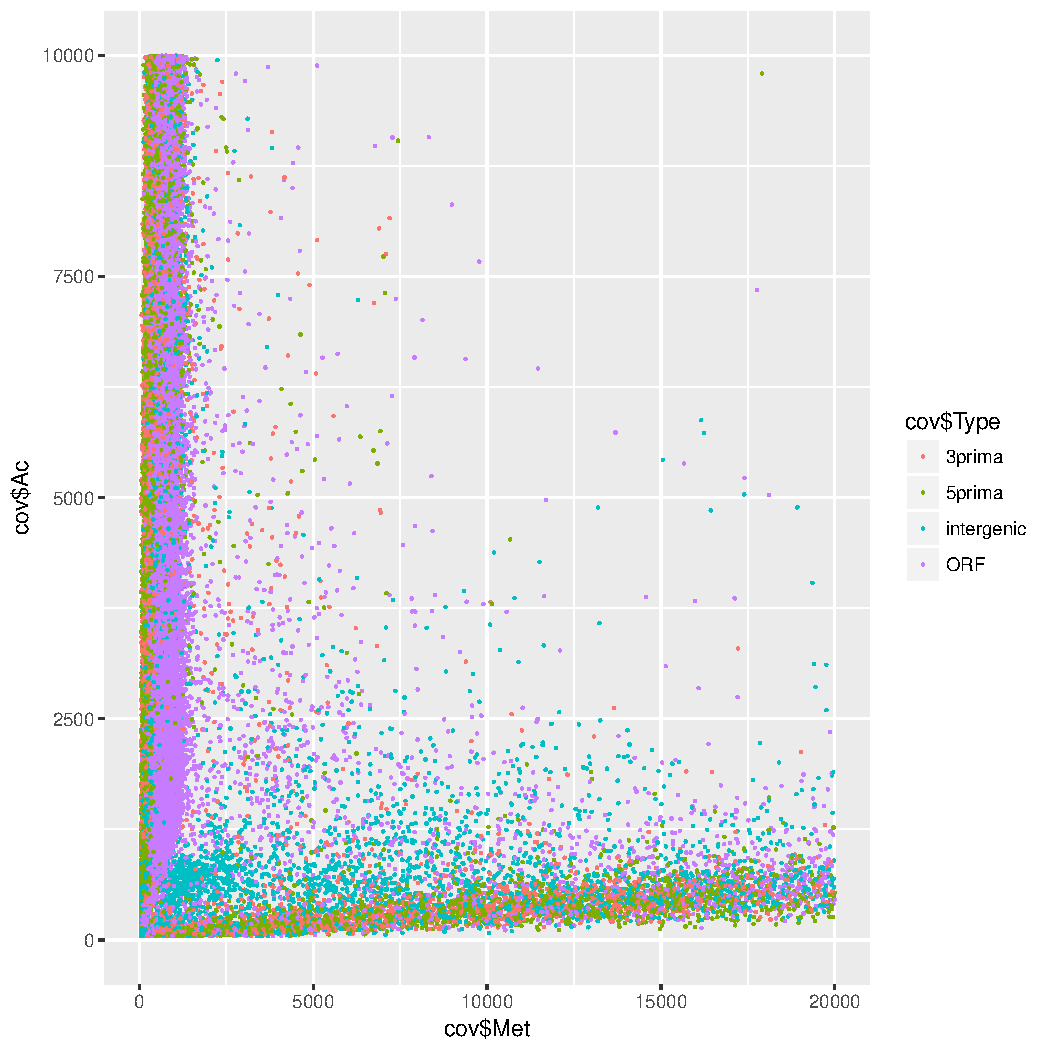
\includegraphics[width=\maxwidth]{figure/unnamed-chunk-1-3} 
\begin{kframe}\begin{alltt}
\hlstd{input_diff[}\hlkwd{abs}\hlstd{(input_diff}\hlopt{$}\hlstd{Gene.cov)} \hlopt{>} \hlnum{1.5}\hlstd{,]}
\end{alltt}
\begin{verbatim}
##       Gene.cov     X5.cov     X3.cov           gene
## 622   1.877972  0.2158246  0.4447963  PF3D7_0400600
## 817  -3.831186 -3.2745906 -4.5699765  PF3D7_0421200
## 818  -2.652479 -0.5715629 -4.5699765  PF3D7_0421300
## 2913  2.766700  1.0067386  3.2878497  PF3D7_1040400
## 2914  3.383116  4.5244806  4.9862657  PF3D7_1040500
## 2915  4.291627  2.5764032  3.1897343  PF3D7_1040600
## 2916  4.422475  3.7654835  3.6358880  PF3D7_1040700
## 2923 -3.928537 -3.4555597 -2.8503676  PF3D7_1100100
## 2924 -1.536825  0.2497792 -2.9827428  PF3D7_1100200
## 5426  2.394479  4.8069478 -0.4805046 PF3D7_API01300
## 5428  5.324187  2.4977887  4.6681096 PF3D7_API01500
## 5429  2.002803  4.6681096  6.3430268 PF3D7_API01600
## 5430  2.691787  6.3430268  8.7615148 PF3D7_API01700
## 5431  6.544474  8.7615148  4.4001629 PF3D7_API01800
## 5432  2.901540  4.4001629  1.8708459 PF3D7_API01900
## 5433  3.548543  4.7117022  2.3840098 PF3D7_API02000
## 5435  1.966285  2.9751021  2.3694832 PF3D7_API02200
## 5436  2.435243  1.6123764 -0.5266608 PF3D7_API02300
## 5437  2.289039 -0.5266608  3.0183883 PF3D7_API02400
## 5438  2.365339  2.3404370  3.1433365 PF3D7_API02500
## 5439  1.529386  2.2317655  3.8154069 PF3D7_API02600
## 5440  4.314276  3.8154069  4.7678951 PF3D7_API02700
## 5441  2.937672  4.7678951  4.5468132 PF3D7_API02800
## 5442  5.214791  4.5468132  4.3748524 PF3D7_API02900
## 5443  2.145038  4.3748524  7.9233844 PF3D7_API03000
## 5444  2.644585  7.9233844  2.3223904 PF3D7_API03500
## 5445  2.986455  4.3990517  3.8136091 PF3D7_API03600
## 5446  3.872340  3.8136091  3.1646520 PF3D7_API03800
## 5447  2.117541  3.1646520  3.1365703 PF3D7_API04000
## 5448  2.397191  1.9960944  2.9354015 PF3D7_API04100
## 5449  2.453248  1.6545512  1.9960944 PF3D7_API04200
## 5450  2.840735  3.4528211  1.6545512 PF3D7_API04300
## 5451  2.628537  1.0570375  3.4528211 PF3D7_API04400
## 5452  1.830456  2.4789126  1.0570375 PF3D7_API04500
## 5454  3.373866  0.6731373  0.8895123 PF3D7_API04700
## 5455 27.219194 25.3769633 22.7577430     mal_mito_1
## 5456 27.356335 25.3769633 29.8731279     mal_mito_2
## 5457 24.444277 29.8731279 25.9053567     mal_mito_3
\end{verbatim}
\begin{alltt}
\hlstd{x} \hlkwb{<-} \hlstd{input_cov[input_cov}\hlopt{$}\hlstd{Gene} \hlopt \hlstd{dif_10G_cov}\hlopt{$}\hlstd{Gene,}\hlnum{1}\hlopt{:}\hlnum{2}\hlstd{]}
\end{alltt}


{\ttfamily\noindent\bfseries\color{errorcolor}{\#\# Error in eval(expr, envir, enclos): object 'input\_cov' not found}}\begin{alltt}
\hlkwd{write.csv}\hlstd{(x,} \hlkwc{file} \hlstd{=} \hlstr{"/home/lucas/ISGlobal/input_cov.csv"}\hlstd{,} \hlkwc{quote} \hlstd{=} \hlnum{FALSE}\hlstd{)}
\end{alltt}


{\ttfamily\noindent\bfseries\color{errorcolor}{\#\# Error in is.data.frame(x): object 'x' not found}}\end{kframe}
\end{knitrout}
  
\end{document}
